The nice people at \emph{The Dispatch} pointed out this
\href{https://web.archive.org/web/20230120124257/https://twitter.com/repandybiggsaz/status/1615419794362142731}{post
to Twitter by Andy Biggs, a congressman from Arizona}:

\begin{figure}
\centering
\pandocbounded{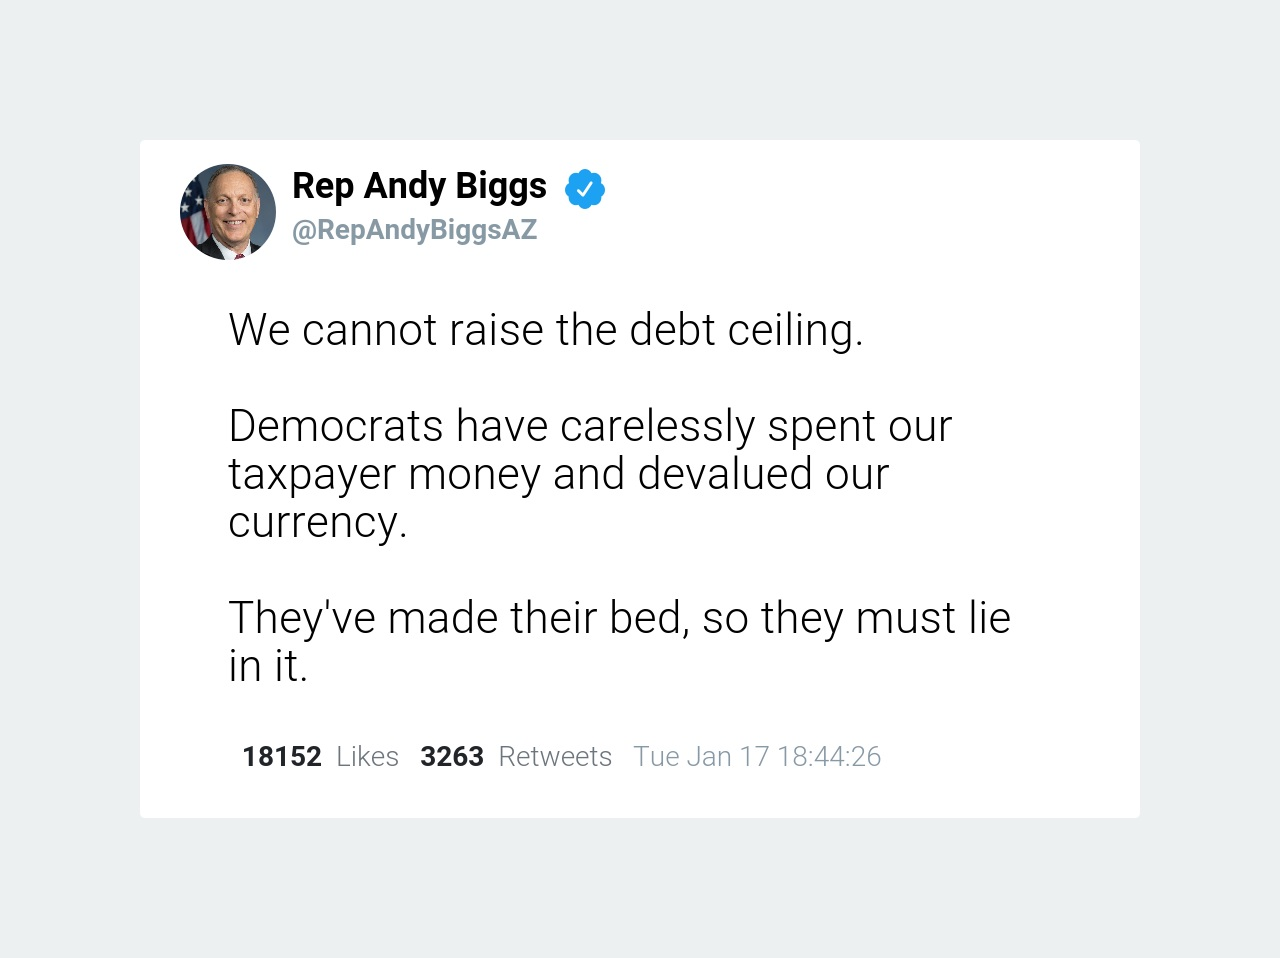
\includegraphics[keepaspectratio]{\%7B\%7Bsite.url\%7D\%7D/img/biggs-destructions.jpg}}
\caption{``We cannot raise the debt ceiling. Democrats have carelessly
spent our taxpayer money and devalued our currency. They've made their
bed, so they must lie in it.''}
\end{figure}

Biggs is a bit of a leader in the House. He can certainly gum up the
works in trying to get a change in the debt ceiling passed. That could
be a problem.

Who are the members of the House Rules Committee? After all, they
control the business on the floor. Members of the committee include:

\begin{itemize}
\tightlist
\item
  Tom Cole (R-OK), Chair
\item
  Michael Burgess (R-TX)
\item
  Guy Reschenthaler (R-PA)
\item
  Michelle Fischbach (R-MN)
\item
  Thomas Massie (R-KY)
\item
  Ralph Norman (R-SC)
\item
  Chip Roy (R-TX)
\item
  Erin Houchin (R-IN)
\item
  Nick Langworthy (R-NY)
\item
  Jim McGovern (D-MA), Ranking Member
\item
  Mary Gay Scanlon (D-PA)
\item
  Joe Neguse (D-CO)
\item
  Teresa Leger Fernandez (D-NM)
\end{itemize}

Only two out of the nine majority party members of the Rules Committee
can be said to be anywhere near centrist/mainstream. Those would be
Michelle Fischbach and Nick Langworthy. The other seven are all varying
degrees of extreme at this point. Any debt deal essentially needs the
agreement of those nine Republicans or it will never make it to the
floor of the House unless it goes through the convoluted time-consuming
procedure of a discharge petition.

Assuming Kevin McCarthy can hold his caucus together he can only lose
\emph{four} votes. I've got at least eight who want to go down the
``Thelma and Louise'' route to varying extents. There are probably more
but with as fractious and bumptious as the caucus appears to be frankly
I don't see a positive way forward to get a deal. Six Republicans
quietly signing a discharge petition in conjunction with all the
Democrats would work but would also end six political careers\ldots{}
